\documentclass[twoside]{book}

% Packages required by doxygen
\usepackage{fixltx2e}
\usepackage{calc}
\usepackage{doxygen}
\usepackage[export]{adjustbox} % also loads graphicx
\usepackage{graphicx}
\usepackage[utf8]{inputenc}
\usepackage{makeidx}
\usepackage{multicol}
\usepackage{multirow}
\PassOptionsToPackage{warn}{textcomp}
\usepackage{textcomp}
\usepackage[nointegrals]{wasysym}
\usepackage[table]{xcolor}

% Font selection
\usepackage[T1]{fontenc}
\usepackage[scaled=.90]{helvet}
\usepackage{courier}
\usepackage{amssymb}
\usepackage{sectsty}
\renewcommand{\familydefault}{\sfdefault}
\allsectionsfont{%
  \fontseries{bc}\selectfont%
  \color{darkgray}%
}
\renewcommand{\DoxyLabelFont}{%
  \fontseries{bc}\selectfont%
  \color{darkgray}%
}
\newcommand{\+}{\discretionary{\mbox{\scriptsize$\hookleftarrow$}}{}{}}

% Page & text layout
\usepackage{geometry}
\geometry{%
  a4paper,%
  top=2.5cm,%
  bottom=2.5cm,%
  left=2.5cm,%
  right=2.5cm%
}
\tolerance=750
\hfuzz=15pt
\hbadness=750
\setlength{\emergencystretch}{15pt}
\setlength{\parindent}{0cm}
\setlength{\parskip}{3ex plus 2ex minus 2ex}
\makeatletter
\renewcommand{\paragraph}{%
  \@startsection{paragraph}{4}{0ex}{-1.0ex}{1.0ex}{%
    \normalfont\normalsize\bfseries\SS@parafont%
  }%
}
\renewcommand{\subparagraph}{%
  \@startsection{subparagraph}{5}{0ex}{-1.0ex}{1.0ex}{%
    \normalfont\normalsize\bfseries\SS@subparafont%
  }%
}
\makeatother

% Headers & footers
\usepackage{fancyhdr}
\pagestyle{fancyplain}
\fancyhead[LE]{\fancyplain{}{\bfseries\thepage}}
\fancyhead[CE]{\fancyplain{}{}}
\fancyhead[RE]{\fancyplain{}{\bfseries\leftmark}}
\fancyhead[LO]{\fancyplain{}{\bfseries\rightmark}}
\fancyhead[CO]{\fancyplain{}{}}
\fancyhead[RO]{\fancyplain{}{\bfseries\thepage}}
\fancyfoot[LE]{\fancyplain{}{}}
\fancyfoot[CE]{\fancyplain{}{}}
\fancyfoot[RE]{\fancyplain{}{\bfseries\scriptsize Generated by Doxygen }}
\fancyfoot[LO]{\fancyplain{}{\bfseries\scriptsize Generated by Doxygen }}
\fancyfoot[CO]{\fancyplain{}{}}
\fancyfoot[RO]{\fancyplain{}{}}
\renewcommand{\footrulewidth}{0.4pt}
\renewcommand{\chaptermark}[1]{%
  \markboth{#1}{}%
}
\renewcommand{\sectionmark}[1]{%
  \markright{\thesection\ #1}%
}

% Indices & bibliography
\usepackage{natbib}
\usepackage[titles]{tocloft}
\setcounter{tocdepth}{3}
\setcounter{secnumdepth}{5}
\makeindex

% Hyperlinks (required, but should be loaded last)
\usepackage{ifpdf}
\ifpdf
  \usepackage[pdftex,pagebackref=true]{hyperref}
\else
  \usepackage[ps2pdf,pagebackref=true]{hyperref}
\fi
\hypersetup{%
  colorlinks=true,%
  linkcolor=blue,%
  citecolor=blue,%
  unicode%
}

% Custom commands
\newcommand{\clearemptydoublepage}{%
  \newpage{\pagestyle{empty}\cleardoublepage}%
}

\usepackage{caption}
\captionsetup{labelsep=space,justification=centering,font={bf},singlelinecheck=off,skip=4pt,position=top}

%===== C O N T E N T S =====

\begin{document}

% Titlepage & ToC
\hypersetup{pageanchor=false,
             bookmarksnumbered=true,
             pdfencoding=unicode
            }
\pagenumbering{alph}
\begin{titlepage}
\vspace*{7cm}
\begin{center}%
{\Large Euler 1D \\[1ex]\large 1.\+0 }\\
\vspace*{1cm}
{\large Generated by Doxygen 1.8.13}\\
\end{center}
\end{titlepage}
\clearemptydoublepage
\pagenumbering{roman}
\tableofcontents
\clearemptydoublepage
\pagenumbering{arabic}
\hypersetup{pageanchor=true}

%--- Begin generated contents ---
\chapter{Namespace Index}
\section{Namespace List}
Here is a list of all documented namespaces with brief descriptions\+:\begin{DoxyCompactList}
\item\contentsline{section}{\hyperlink{namespaceEu1D}{Eu1D} \\*Namespace to hold all necesary constants }{\pageref{namespaceEu1D}}{}
\end{DoxyCompactList}

\chapter{Class Index}
\section{Class List}
Here are the classes, structs, unions and interfaces with brief descriptions\+:\begin{DoxyCompactList}
\item\contentsline{section}{\hyperlink{classEuler1D}{Euler1D} }{\pageref{classEuler1D}}{}
\item\contentsline{section}{\hyperlink{classgridFunc1D}{grid\+Func1D} }{\pageref{classgridFunc1D}}{}
\item\contentsline{section}{\hyperlink{classmVector}{m\+Vector$<$ T $>$} }{\pageref{classmVector}}{}
\item\contentsline{section}{\hyperlink{classparameterReader}{parameter\+Reader} }{\pageref{classparameterReader}}{}
\item\contentsline{section}{\hyperlink{classSimulation}{Simulation} }{\pageref{classSimulation}}{}
\item\contentsline{section}{\hyperlink{classTimeIntegrator}{Time\+Integrator} }{\pageref{classTimeIntegrator}}{}
\end{DoxyCompactList}

\chapter{Namespace Documentation}
\hypertarget{namespaceEu1D}{}\section{Eu1D Namespace Reference}
\label{namespaceEu1D}\index{Eu1D@{Eu1D}}


Namespace to hold all necesary constants.  


\subsection*{Variables}
\begin{DoxyCompactItemize}
\item 
\mbox{\Hypertarget{namespaceEu1D_a11c0e40fc3c8e0bfa0fdddf6ff676661}\label{namespaceEu1D_a11c0e40fc3c8e0bfa0fdddf6ff676661}} 
const double {\bfseries gam} = 5.\+0/3.\+0
\end{DoxyCompactItemize}


\subsection{Detailed Description}
Namespace to hold all necesary constants. 
\chapter{Class Documentation}
\hypertarget{classEuler1D}{}\section{Euler1D Class Reference}
\label{classEuler1D}\index{Euler1D@{Euler1D}}


Collaboration diagram for Euler1D\+:
\nopagebreak
\begin{figure}[H]
\begin{center}
\leavevmode
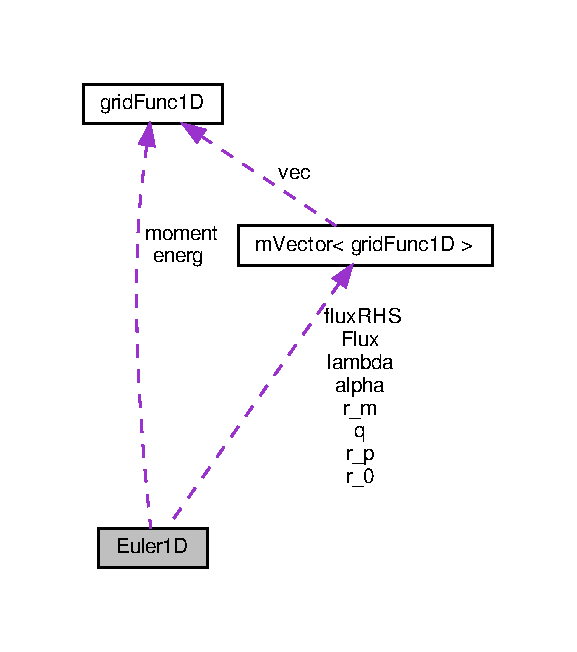
\includegraphics[width=277pt]{classEuler1D__coll__graph}
\end{center}
\end{figure}
\subsection*{Public Member Functions}
\begin{DoxyCompactItemize}
\item 
\mbox{\Hypertarget{classEuler1D_ad84569261342179e02254ea816ee15c0}\label{classEuler1D_ad84569261342179e02254ea816ee15c0}} 
\hyperlink{classEuler1D_ad84569261342179e02254ea816ee15c0}{Euler1D} (const \hyperlink{classparameterReader}{parameter\+Reader} \&p)
\begin{DoxyCompactList}\small\item\em q is a \hyperlink{classmVector}{m\+Vector} that hold the variables q\mbox{[}0\mbox{]} is the density q\mbox{[}1\mbox{]} is velocity q\mbox{[}2\mbox{]} is pressure \end{DoxyCompactList}\item 
\mbox{\Hypertarget{classEuler1D_ad1612560c24dc0bb0aa54b2bc65bfade}\label{classEuler1D_ad1612560c24dc0bb0aa54b2bc65bfade}} 
\hyperlink{classmVector}{m\+Vector}$<$ \hyperlink{classgridFunc1D}{grid\+Func1D} $>$ \& {\bfseries state\+Vector} ()
\item 
\mbox{\Hypertarget{classEuler1D_a939370b2721b7ac97053e4ea95ee5cb9}\label{classEuler1D_a939370b2721b7ac97053e4ea95ee5cb9}} 
const \hyperlink{classgridFunc1D}{grid\+Func1D} \& {\bfseries density} () const
\item 
\mbox{\Hypertarget{classEuler1D_ae81f6e2348124ef702a9257ae512a750}\label{classEuler1D_ae81f6e2348124ef702a9257ae512a750}} 
const \hyperlink{classgridFunc1D}{grid\+Func1D} \& {\bfseries vel} () const
\item 
\mbox{\Hypertarget{classEuler1D_a9046ccec8f4ecc822c260dfd3050ceb8}\label{classEuler1D_a9046ccec8f4ecc822c260dfd3050ceb8}} 
const \hyperlink{classgridFunc1D}{grid\+Func1D} \& {\bfseries pres} () const
\item 
\mbox{\Hypertarget{classEuler1D_a146d711f6675812bfec8dbc791503753}\label{classEuler1D_a146d711f6675812bfec8dbc791503753}} 
const \hyperlink{classgridFunc1D}{grid\+Func1D} \& {\bfseries momentum} ()
\item 
\mbox{\Hypertarget{classEuler1D_aa4d4e90fbf535fe877a87695d45555d4}\label{classEuler1D_aa4d4e90fbf535fe877a87695d45555d4}} 
const \hyperlink{classgridFunc1D}{grid\+Func1D} \& {\bfseries energy} ()
\item 
\mbox{\Hypertarget{classEuler1D_aea503a1e62ad484ca74b04da1b4c9300}\label{classEuler1D_aea503a1e62ad484ca74b04da1b4c9300}} 
void \hyperlink{classEuler1D_aea503a1e62ad484ca74b04da1b4c9300}{initial\+Data} (\hyperlink{classgridFunc1D}{grid\+Func1D} \&x, const \hyperlink{classparameterReader}{parameter\+Reader} \&p)
\begin{DoxyCompactList}\small\item\em Four types of shock tubes as initial data. \end{DoxyCompactList}\item 
\hyperlink{classmVector}{m\+Vector}$<$ \hyperlink{classgridFunc1D}{grid\+Func1D} $>$ \hyperlink{classEuler1D_a466e76f0be22e407e3b17072fb567fb4}{R\+HS} (const \hyperlink{classmVector}{m\+Vector}$<$ \hyperlink{classgridFunc1D}{grid\+Func1D} $>$ \&iq, double dx)
\begin{DoxyCompactList}\small\item\em Evolve in time from t to t+dt. \end{DoxyCompactList}\item 
\mbox{\Hypertarget{classEuler1D_a994704a8f516533966aa368bc6b34682}\label{classEuler1D_a994704a8f516533966aa368bc6b34682}} 
void {\bfseries output} (\hyperlink{classgridFunc1D}{grid\+Func1D} \&x, double t)
\end{DoxyCompactItemize}
\subsection*{Private Attributes}
\begin{DoxyCompactItemize}
\item 
\mbox{\Hypertarget{classEuler1D_a4d7ee173fabfdf028c3658607edfb706}\label{classEuler1D_a4d7ee173fabfdf028c3658607edfb706}} 
\hyperlink{classmVector}{m\+Vector}$<$ \hyperlink{classgridFunc1D}{grid\+Func1D} $>$ {\bfseries q}
\item 
\mbox{\Hypertarget{classEuler1D_a0119979b53cf0ddcd45dd1a409d14ee8}\label{classEuler1D_a0119979b53cf0ddcd45dd1a409d14ee8}} 
\hyperlink{classmVector}{m\+Vector}$<$ \hyperlink{classgridFunc1D}{grid\+Func1D} $>$ {\bfseries Flux}
\item 
\mbox{\Hypertarget{classEuler1D_a8dd5ef79e3aafaf95e7cf60f122e18de}\label{classEuler1D_a8dd5ef79e3aafaf95e7cf60f122e18de}} 
\hyperlink{classmVector}{m\+Vector}$<$ \hyperlink{classgridFunc1D}{grid\+Func1D} $>$ {\bfseries r\+\_\+m}
\item 
\mbox{\Hypertarget{classEuler1D_aca17997549fc42c1787bf1cf4c709484}\label{classEuler1D_aca17997549fc42c1787bf1cf4c709484}} 
\hyperlink{classmVector}{m\+Vector}$<$ \hyperlink{classgridFunc1D}{grid\+Func1D} $>$ {\bfseries r\+\_\+0}
\item 
\mbox{\Hypertarget{classEuler1D_a86e407119b0789ab0dc475b9acd2097d}\label{classEuler1D_a86e407119b0789ab0dc475b9acd2097d}} 
\hyperlink{classmVector}{m\+Vector}$<$ \hyperlink{classgridFunc1D}{grid\+Func1D} $>$ {\bfseries r\+\_\+p}
\item 
\mbox{\Hypertarget{classEuler1D_ad68269f3b44c914a5b51b5b6a3aa8910}\label{classEuler1D_ad68269f3b44c914a5b51b5b6a3aa8910}} 
\hyperlink{classmVector}{m\+Vector}$<$ \hyperlink{classgridFunc1D}{grid\+Func1D} $>$ {\bfseries alpha}
\item 
\mbox{\Hypertarget{classEuler1D_ae7c0ed4ec766896cb5a20ebca877d08f}\label{classEuler1D_ae7c0ed4ec766896cb5a20ebca877d08f}} 
\hyperlink{classmVector}{m\+Vector}$<$ \hyperlink{classgridFunc1D}{grid\+Func1D} $>$ {\bfseries lambda}
\item 
\mbox{\Hypertarget{classEuler1D_a7056e02d1f1c8e228441d39384e2638d}\label{classEuler1D_a7056e02d1f1c8e228441d39384e2638d}} 
\hyperlink{classmVector}{m\+Vector}$<$ \hyperlink{classgridFunc1D}{grid\+Func1D} $>$ {\bfseries flux\+R\+HS}
\item 
\mbox{\Hypertarget{classEuler1D_ad3a4ed7f5c1279905f28e91bac38fd59}\label{classEuler1D_ad3a4ed7f5c1279905f28e91bac38fd59}} 
\hyperlink{classgridFunc1D}{grid\+Func1D} {\bfseries moment}
\item 
\mbox{\Hypertarget{classEuler1D_a06ded8b55a4416e73e92cbbed4c74411}\label{classEuler1D_a06ded8b55a4416e73e92cbbed4c74411}} 
\hyperlink{classgridFunc1D}{grid\+Func1D} {\bfseries energ}
\item 
\mbox{\Hypertarget{classEuler1D_af7770027091036a697ab97030e9bbe9e}\label{classEuler1D_af7770027091036a697ab97030e9bbe9e}} 
int {\bfseries conv\+Factor}
\end{DoxyCompactItemize}


\subsection{Detailed Description}


Definition at line 7 of file Euler1\+D.\+hpp.



\subsection{Member Function Documentation}
\mbox{\Hypertarget{classEuler1D_a466e76f0be22e407e3b17072fb567fb4}\label{classEuler1D_a466e76f0be22e407e3b17072fb567fb4}} 
\index{Euler1D@{Euler1D}!R\+HS@{R\+HS}}
\index{R\+HS@{R\+HS}!Euler1D@{Euler1D}}
\subsubsection{\texorpdfstring{R\+H\+S()}{RHS()}}
{\footnotesize\ttfamily \hyperlink{classmVector}{m\+Vector}$<$ \hyperlink{classgridFunc1D}{grid\+Func1D} $>$ Euler1\+D\+::\+R\+HS (\begin{DoxyParamCaption}\item[{const \hyperlink{classmVector}{m\+Vector}$<$ \hyperlink{classgridFunc1D}{grid\+Func1D} $>$ \&}]{iq,  }\item[{double}]{dx }\end{DoxyParamCaption})}



Evolve in time from t to t+dt. 

This is the most simple thing we can do. It is a first order method 

Definition at line 170 of file Euler1\+D.\+cpp.


\begin{DoxyCode}
171 \{
172   \textcolor{comment}{// iq stands for input q}
173   \textcolor{keyword}{const} \textcolor{keywordtype}{int} N = iq[0].Npoints();
174   
175   calcFlux3( iq, alpha, r\_m, r\_0, r\_p, lambda, Flux );
176   
177   \textcolor{comment}{// compute net fluxes}
178   \textcolor{keywordflow}{for}( \textcolor{keywordtype}{int} i=3; i<=N-2; i++ )\{
179     fluxRHS[0][i] = -( Flux[0][i+1] - Flux[0][i] )/dx;
180     fluxRHS[1][i] = -( Flux[1][i+1] - Flux[1][i] )/dx;
181     fluxRHS[2][i] = -( Flux[2][i+1] - Flux[2][i] )/dx;
182   \}
183 
184   \textcolor{keywordflow}{return} fluxRHS;
185 \}
\end{DoxyCode}


The documentation for this class was generated from the following files\+:\begin{DoxyCompactItemize}
\item 
Euler1\+D.\+hpp\item 
Euler1\+D.\+cpp\end{DoxyCompactItemize}

\hypertarget{classgridFunc1D}{}\section{grid\+Func1D Class Reference}
\label{classgridFunc1D}\index{grid\+Func1D@{grid\+Func1D}}
\subsection*{Public Member Functions}
\begin{DoxyCompactItemize}
\item 
\hyperlink{classgridFunc1D_a014ccb9f69e514547d24998fd3f5523b}{grid\+Func1D} ()
\begin{DoxyCompactList}\small\item\em Constructor with no arguments. \end{DoxyCompactList}\item 
\mbox{\Hypertarget{classgridFunc1D_a3f83c015b602a1d4ea0a0b9bf00812bd}\label{classgridFunc1D_a3f83c015b602a1d4ea0a0b9bf00812bd}} 
\hyperlink{classgridFunc1D_a3f83c015b602a1d4ea0a0b9bf00812bd}{grid\+Func1D} (int)
\begin{DoxyCompactList}\small\item\em Initializes and creates space to hold n elements. \end{DoxyCompactList}\item 
\mbox{\Hypertarget{classgridFunc1D_a3e5e1b42909e666b2d996a2c7b20124d}\label{classgridFunc1D_a3e5e1b42909e666b2d996a2c7b20124d}} 
\hyperlink{classgridFunc1D_a3e5e1b42909e666b2d996a2c7b20124d}{grid\+Func1D} (const \hyperlink{classgridFunc1D}{grid\+Func1D} \&)
\begin{DoxyCompactList}\small\item\em Copy constructor. \end{DoxyCompactList}\item 
void \hyperlink{classgridFunc1D_a0d33423ea192c516bfaf9c0cc77cd943}{create} (int)
\begin{DoxyCompactList}\small\item\em Creates and resize the objects. \end{DoxyCompactList}\item 
\mbox{\Hypertarget{classgridFunc1D_a4df1b6d0de38c1d13e2cfc473d77cb5d}\label{classgridFunc1D_a4df1b6d0de38c1d13e2cfc473d77cb5d}} 
void {\bfseries erase} ()
\item 
\mbox{\Hypertarget{classgridFunc1D_a4bea39799321d46142b978a8a17d800e}\label{classgridFunc1D_a4bea39799321d46142b978a8a17d800e}} 
double \& {\bfseries operator\mbox{[}$\,$\mbox{]}} (float) const
\item 
\mbox{\Hypertarget{classgridFunc1D_a5c270cddc809aa94b3dfce3588b8aacd}\label{classgridFunc1D_a5c270cddc809aa94b3dfce3588b8aacd}} 
double \& {\bfseries operator\mbox{[}$\,$\mbox{]}} (float)
\item 
\mbox{\Hypertarget{classgridFunc1D_a71aaccb7ea0b40b0360afdf398d07fa0}\label{classgridFunc1D_a71aaccb7ea0b40b0360afdf398d07fa0}} 
int \hyperlink{classgridFunc1D_a71aaccb7ea0b40b0360afdf398d07fa0}{Npoints} () const
\begin{DoxyCompactList}\small\item\em Get the number of points. \end{DoxyCompactList}\item 
\mbox{\Hypertarget{classgridFunc1D_a83347f8764f77eef88ef326ef71d96b3}\label{classgridFunc1D_a83347f8764f77eef88ef326ef71d96b3}} 
void {\bfseries set\+Boundary\+Condition} (int)
\item 
\mbox{\Hypertarget{classgridFunc1D_aba748038bbce60927dd328ebe5f712ac}\label{classgridFunc1D_aba748038bbce60927dd328ebe5f712ac}} 
void {\bfseries set\+Is\+Flux} (int)
\item 
void \hyperlink{classgridFunc1D_a5dc63c77c8be317834291dcd0d66079d}{output\+Gnuplot\+Fake} (ofstream \&, \hyperlink{classgridFunc1D}{grid\+Func1D} \&, const double)
\begin{DoxyCompactList}\small\item\em Gnuplot style output (fake) \end{DoxyCompactList}\item 
void \hyperlink{classgridFunc1D_aeb63f2e7e15429025c33aa24abf288ad}{output\+Gnuplot} (ofstream \&, \hyperlink{classgridFunc1D}{grid\+Func1D} \&, const double) const
\begin{DoxyCompactList}\small\item\em Gnuplot style output. \end{DoxyCompactList}\item 
void \hyperlink{classgridFunc1D_a07793d54b659a46c6a38c3fe0b70f6c2}{output\+By\+Line} (ofstream \&, const double t) const
\begin{DoxyCompactList}\small\item\em Output all the values of the variable in a single line. \end{DoxyCompactList}\item 
void \hyperlink{classgridFunc1D_a9843d7697659ce644eb46c127f9c57cb}{output\+By\+Column} (ofstream \&, \hyperlink{classgridFunc1D}{grid\+Func1D} \&, const double t) const
\begin{DoxyCompactList}\small\item\em ygraph output style \end{DoxyCompactList}\item 
\mbox{\Hypertarget{classgridFunc1D_a121a7d446c2cfbfbbfc685ccc70c3e30}\label{classgridFunc1D_a121a7d446c2cfbfbbfc685ccc70c3e30}} 
\hyperlink{classgridFunc1D}{grid\+Func1D} {\bfseries operator+} (const \hyperlink{classgridFunc1D}{grid\+Func1D} \&B) const
\item 
\mbox{\Hypertarget{classgridFunc1D_a18dc29bb1beca6f09ab507ced3f5ff50}\label{classgridFunc1D_a18dc29bb1beca6f09ab507ced3f5ff50}} 
\hyperlink{classgridFunc1D}{grid\+Func1D} {\bfseries operator-\/} (const \hyperlink{classgridFunc1D}{grid\+Func1D} \&B) const
\item 
\mbox{\Hypertarget{classgridFunc1D_a6143c22e1c52a94b7618a9478e44b6c9}\label{classgridFunc1D_a6143c22e1c52a94b7618a9478e44b6c9}} 
\hyperlink{classgridFunc1D}{grid\+Func1D} {\bfseries operator$\ast$} (const \hyperlink{classgridFunc1D}{grid\+Func1D} \&B) const
\item 
\mbox{\Hypertarget{classgridFunc1D_a4415608c844ce3098e09df36c31ad6c5}\label{classgridFunc1D_a4415608c844ce3098e09df36c31ad6c5}} 
\hyperlink{classgridFunc1D}{grid\+Func1D} {\bfseries operator$\ast$} (const double \&b) const
\item 
\mbox{\Hypertarget{classgridFunc1D_ae21f476b7a1c40a4fcf013e20efef31a}\label{classgridFunc1D_ae21f476b7a1c40a4fcf013e20efef31a}} 
\hyperlink{classgridFunc1D}{grid\+Func1D} {\bfseries operator/} (const double \&b) const
\item 
\mbox{\Hypertarget{classgridFunc1D_a3c852d13b415f5c167a50bca0ea14124}\label{classgridFunc1D_a3c852d13b415f5c167a50bca0ea14124}} 
\hyperlink{classgridFunc1D}{grid\+Func1D} {\bfseries operator/} (const \hyperlink{classgridFunc1D}{grid\+Func1D} \&B) const
\item 
\mbox{\Hypertarget{classgridFunc1D_a0bf1365b51d3f71b36877cd7ce7aaa6a}\label{classgridFunc1D_a0bf1365b51d3f71b36877cd7ce7aaa6a}} 
const \hyperlink{classgridFunc1D}{grid\+Func1D} \& {\bfseries operator=} (const \hyperlink{classgridFunc1D}{grid\+Func1D} \&B)
\item 
\mbox{\Hypertarget{classgridFunc1D_ac9c3bd3b43873d9e0ba174e1010d5188}\label{classgridFunc1D_ac9c3bd3b43873d9e0ba174e1010d5188}} 
const \hyperlink{classgridFunc1D}{grid\+Func1D} \& {\bfseries operator=} (const double b)
\item 
\mbox{\Hypertarget{classgridFunc1D_a72cf64cc9788b269c3830a1a1c6a55f2}\label{classgridFunc1D_a72cf64cc9788b269c3830a1a1c6a55f2}} 
const \hyperlink{classgridFunc1D}{grid\+Func1D} \& {\bfseries operator=} (const int b)
\item 
\mbox{\Hypertarget{classgridFunc1D_a6eb98fafdb29757160e503415e49a0ca}\label{classgridFunc1D_a6eb98fafdb29757160e503415e49a0ca}} 
void \hyperlink{classgridFunc1D_a6eb98fafdb29757160e503415e49a0ca}{ishuge} (double a)
\begin{DoxyCompactList}\small\item\em Checks is a given value is greater than a. \end{DoxyCompactList}\end{DoxyCompactItemize}
\subsection*{Private Attributes}
\begin{DoxyCompactItemize}
\item 
\mbox{\Hypertarget{classgridFunc1D_a4ababbcbdca2a233cb673fc8b1997ad1}\label{classgridFunc1D_a4ababbcbdca2a233cb673fc8b1997ad1}} 
int {\bfseries n\+\_\+points}
\item 
\mbox{\Hypertarget{classgridFunc1D_a2d4e4f9d31f1ae7406354bfd4c5a9db5}\label{classgridFunc1D_a2d4e4f9d31f1ae7406354bfd4c5a9db5}} 
double $\ast$ {\bfseries data}
\item 
\mbox{\Hypertarget{classgridFunc1D_a4bd8aa8cca871f1183ae3f2cb735f909}\label{classgridFunc1D_a4bd8aa8cca871f1183ae3f2cb735f909}} 
double $\ast$ {\bfseries datamid}
\item 
\mbox{\Hypertarget{classgridFunc1D_a7ca7772f4f7efcbd9e686bf292779433}\label{classgridFunc1D_a7ca7772f4f7efcbd9e686bf292779433}} 
int {\bfseries boundary\+Type}
\item 
\mbox{\Hypertarget{classgridFunc1D_a8b4a9154c3cfa2756353bf62f1440821}\label{classgridFunc1D_a8b4a9154c3cfa2756353bf62f1440821}} 
int {\bfseries is\+Flux}
\end{DoxyCompactItemize}
\subsection*{Friends}
\begin{DoxyCompactItemize}
\item 
\mbox{\Hypertarget{classgridFunc1D_a82f5077526c231d53777ffa8dc25babe}\label{classgridFunc1D_a82f5077526c231d53777ffa8dc25babe}} 
\hyperlink{classgridFunc1D}{grid\+Func1D} {\bfseries operator-\/} (const double a, const \hyperlink{classgridFunc1D}{grid\+Func1D} \&B)
\item 
\mbox{\Hypertarget{classgridFunc1D_aca721beab66aeb7beaca902c6de6297d}\label{classgridFunc1D_aca721beab66aeb7beaca902c6de6297d}} 
\hyperlink{classgridFunc1D}{grid\+Func1D} {\bfseries operator$\ast$} (const double \&a, const \hyperlink{classgridFunc1D}{grid\+Func1D} \&B)
\item 
\mbox{\Hypertarget{classgridFunc1D_a14fa7624f830d55e478316b887fc1a22}\label{classgridFunc1D_a14fa7624f830d55e478316b887fc1a22}} 
\hyperlink{classgridFunc1D}{grid\+Func1D} {\bfseries operator/} (const double a, const \hyperlink{classgridFunc1D}{grid\+Func1D} \&B)
\item 
\mbox{\Hypertarget{classgridFunc1D_a3a2a38cf32f17dc89c19094b1ae9795a}\label{classgridFunc1D_a3a2a38cf32f17dc89c19094b1ae9795a}} 
\hyperlink{classgridFunc1D}{grid\+Func1D} {\bfseries sqrt} (const \hyperlink{classgridFunc1D}{grid\+Func1D} \&A)
\end{DoxyCompactItemize}


\subsection{Detailed Description}


Definition at line 13 of file grid\+Func1\+D.\+hpp.



\subsection{Constructor \& Destructor Documentation}
\mbox{\Hypertarget{classgridFunc1D_a014ccb9f69e514547d24998fd3f5523b}\label{classgridFunc1D_a014ccb9f69e514547d24998fd3f5523b}} 
\index{grid\+Func1D@{grid\+Func1D}!grid\+Func1D@{grid\+Func1D}}
\index{grid\+Func1D@{grid\+Func1D}!grid\+Func1D@{grid\+Func1D}}
\subsubsection{\texorpdfstring{grid\+Func1\+D()}{gridFunc1D()}}
{\footnotesize\ttfamily grid\+Func1\+D\+::grid\+Func1D (\begin{DoxyParamCaption}{ }\end{DoxyParamCaption})}



Constructor with no arguments. 

It initializes everything to zero 

Definition at line 8 of file grid\+Func1\+D.\+cpp.


\begin{DoxyCode}
9 \{
10   n\_points = 0;
11   data = NULL;
12   datamid = NULL;
13   boundaryType = -1;
14   isFlux = 0;
15 \}
\end{DoxyCode}


\subsection{Member Function Documentation}
\mbox{\Hypertarget{classgridFunc1D_a0d33423ea192c516bfaf9c0cc77cd943}\label{classgridFunc1D_a0d33423ea192c516bfaf9c0cc77cd943}} 
\index{grid\+Func1D@{grid\+Func1D}!create@{create}}
\index{create@{create}!grid\+Func1D@{grid\+Func1D}}
\subsubsection{\texorpdfstring{create()}{create()}}
{\footnotesize\ttfamily void grid\+Func1\+D\+::create (\begin{DoxyParamCaption}\item[{int}]{n }\end{DoxyParamCaption})}



Creates and resize the objects. 

This function assigns space and also can resize an already existing object 

Definition at line 55 of file grid\+Func1\+D.\+cpp.


\begin{DoxyCode}
56 \{
57   erase();
58 
59   \textcolor{keywordflow}{if} ( n > 0 )\{
60     n\_points = n;
61     data = \textcolor{keyword}{new} \textcolor{keywordtype}{double}[n];
62     datamid = \textcolor{keyword}{new} \textcolor{keywordtype}{double}[n+1];
63 
64     \textcolor{keywordflow}{for}( \textcolor{keywordtype}{int} i=0; i<n; i++ )   data[i] = 0.0;
65     \textcolor{keywordflow}{for}( \textcolor{keywordtype}{int} i=0; i<n+1; i++ ) datamid[i] = 0.0;
66   \}
67   \textcolor{keywordflow}{else} \{
68     cout << \textcolor{stringliteral}{"ERROR: the number of points must be positive."}<<endl;
69     exit(1);
70   \}
71 \}
\end{DoxyCode}
\mbox{\Hypertarget{classgridFunc1D_a9843d7697659ce644eb46c127f9c57cb}\label{classgridFunc1D_a9843d7697659ce644eb46c127f9c57cb}} 
\index{grid\+Func1D@{grid\+Func1D}!output\+By\+Column@{output\+By\+Column}}
\index{output\+By\+Column@{output\+By\+Column}!grid\+Func1D@{grid\+Func1D}}
\subsubsection{\texorpdfstring{output\+By\+Column()}{outputByColumn()}}
{\footnotesize\ttfamily void grid\+Func1\+D\+::output\+By\+Column (\begin{DoxyParamCaption}\item[{ofstream \&}]{out,  }\item[{\hyperlink{classgridFunc1D}{grid\+Func1D} \&}]{x,  }\item[{const double}]{t }\end{DoxyParamCaption}) const}



ygraph output style 

ygraph output style consists in starting a block with the current time followed with the position and the value of the variable in one line 

Definition at line 168 of file grid\+Func1\+D.\+cpp.


\begin{DoxyCode}
169 \{
170   out << \textcolor{stringliteral}{"#time = "} << t << endl;
171 
172   \textcolor{keywordflow}{for}( \textcolor{keywordtype}{int} i=1; i<=n\_points; i++ )
173     out << x[i] << \textcolor{stringliteral}{"\(\backslash\)t"} << std::setprecision(15) << (*this)[i] << endl;
174 
175   out << endl;
176 \}
\end{DoxyCode}
\mbox{\Hypertarget{classgridFunc1D_a07793d54b659a46c6a38c3fe0b70f6c2}\label{classgridFunc1D_a07793d54b659a46c6a38c3fe0b70f6c2}} 
\index{grid\+Func1D@{grid\+Func1D}!output\+By\+Line@{output\+By\+Line}}
\index{output\+By\+Line@{output\+By\+Line}!grid\+Func1D@{grid\+Func1D}}
\subsubsection{\texorpdfstring{output\+By\+Line()}{outputByLine()}}
{\footnotesize\ttfamily void grid\+Func1\+D\+::output\+By\+Line (\begin{DoxyParamCaption}\item[{ofstream \&}]{out,  }\item[{const double}]{t }\end{DoxyParamCaption}) const}



Output all the values of the variable in a single line. 

Time is in the first column followed by all the pointwise values of the variable. The position is not output. This is useful the integrate the velocity to get the position of hypothetical particles. 

Definition at line 152 of file grid\+Func1\+D.\+cpp.


\begin{DoxyCode}
153 \{
154   out << t;
155 
156   \textcolor{keywordflow}{for}( \textcolor{keywordtype}{int} i=1; i<=n\_points; i++ )
157     out << \textcolor{stringliteral}{"\(\backslash\)t"} << (*\textcolor{keyword}{this})[i];
158 
159   out << endl;
160 \}
\end{DoxyCode}
\mbox{\Hypertarget{classgridFunc1D_aeb63f2e7e15429025c33aa24abf288ad}\label{classgridFunc1D_aeb63f2e7e15429025c33aa24abf288ad}} 
\index{grid\+Func1D@{grid\+Func1D}!output\+Gnuplot@{output\+Gnuplot}}
\index{output\+Gnuplot@{output\+Gnuplot}!grid\+Func1D@{grid\+Func1D}}
\subsubsection{\texorpdfstring{output\+Gnuplot()}{outputGnuplot()}}
{\footnotesize\ttfamily void grid\+Func1\+D\+::output\+Gnuplot (\begin{DoxyParamCaption}\item[{ofstream \&}]{out,  }\item[{\hyperlink{classgridFunc1D}{grid\+Func1D} \&}]{x,  }\item[{const double}]{t }\end{DoxyParamCaption}) const}



Gnuplot style output. 

First column is time, second column is spatial variable and third column is the field itself 

Definition at line 134 of file grid\+Func1\+D.\+cpp.


\begin{DoxyCode}
135 \{
136   \textcolor{keywordflow}{for}( \textcolor{keywordtype}{int} i=1; i<=n\_points; i++ )
137     out << t << \textcolor{stringliteral}{"\(\backslash\)t"} << x[i] << \textcolor{stringliteral}{"\(\backslash\)t"} << (*\textcolor{keyword}{this})[i] << endl;
138 
139   out << endl << endl;
140 \}
\end{DoxyCode}
\mbox{\Hypertarget{classgridFunc1D_a5dc63c77c8be317834291dcd0d66079d}\label{classgridFunc1D_a5dc63c77c8be317834291dcd0d66079d}} 
\index{grid\+Func1D@{grid\+Func1D}!output\+Gnuplot\+Fake@{output\+Gnuplot\+Fake}}
\index{output\+Gnuplot\+Fake@{output\+Gnuplot\+Fake}!grid\+Func1D@{grid\+Func1D}}
\subsubsection{\texorpdfstring{output\+Gnuplot\+Fake()}{outputGnuplotFake()}}
{\footnotesize\ttfamily void grid\+Func1\+D\+::output\+Gnuplot\+Fake (\begin{DoxyParamCaption}\item[{ofstream \&}]{out,  }\item[{\hyperlink{classgridFunc1D}{grid\+Func1D} \&}]{x,  }\item[{const double}]{t }\end{DoxyParamCaption})}



Gnuplot style output (fake) 

This function is trick to make a 1D variable look like a 2D one. Its purpose is the make a density plot with Gnuplot 

Definition at line 112 of file grid\+Func1\+D.\+cpp.


\begin{DoxyCode}
113 \{
114   out << \textcolor{stringliteral}{"#time = "} << t << endl;
115 
116   \textcolor{keywordflow}{for}( \textcolor{keywordtype}{int} i=1; i<=n\_points; i++ )
117     out << 0.0 << \textcolor{stringliteral}{"\(\backslash\)t"} << x[i] << \textcolor{stringliteral}{"\(\backslash\)t"} << (*\textcolor{keyword}{this})[i] << endl;
118 
119   out << endl;
120 
121   \textcolor{keywordflow}{for}( \textcolor{keywordtype}{int} i=1; i<=n\_points; i++ )
122     out << 1.0 << \textcolor{stringliteral}{"\(\backslash\)t"} << x[i] << \textcolor{stringliteral}{"\(\backslash\)t"} << (*\textcolor{keyword}{this})[i] << endl;
123 
124   out << endl << endl;
125 \}
\end{DoxyCode}


The documentation for this class was generated from the following files\+:\begin{DoxyCompactItemize}
\item 
grid\+Func1\+D.\+hpp\item 
grid\+Func1\+D.\+cpp\end{DoxyCompactItemize}

\hypertarget{classmVector}{}\section{m\+Vector$<$ T $>$ Class Template Reference}
\label{classmVector}\index{m\+Vector$<$ T $>$@{m\+Vector$<$ T $>$}}


Collaboration diagram for m\+Vector$<$ T $>$\+:
\nopagebreak
\begin{figure}[H]
\begin{center}
\leavevmode
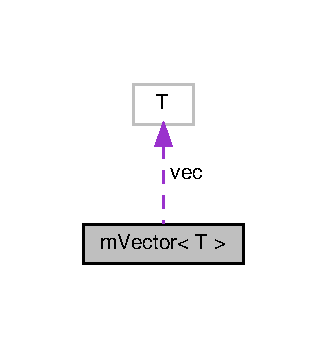
\includegraphics[width=157pt]{classmVector__coll__graph}
\end{center}
\end{figure}
\subsection*{Public Member Functions}
\begin{DoxyCompactItemize}
\item 
\mbox{\Hypertarget{classmVector_a5aad638cf6e1cde4ea630ba1235b6d4e}\label{classmVector_a5aad638cf6e1cde4ea630ba1235b6d4e}} 
\hyperlink{classmVector_a5aad638cf6e1cde4ea630ba1235b6d4e}{m\+Vector} ()
\begin{DoxyCompactList}\small\item\em Constructor. \end{DoxyCompactList}\item 
\mbox{\Hypertarget{classmVector_a8c7b3bad50a6ced368ee66707733933c}\label{classmVector_a8c7b3bad50a6ced368ee66707733933c}} 
{\bfseries m\+Vector} (int)
\item 
\mbox{\Hypertarget{classmVector_a3f49c8d14ab7d7d87e61dc2b42e82108}\label{classmVector_a3f49c8d14ab7d7d87e61dc2b42e82108}} 
void {\bfseries resize} (int)
\item 
\mbox{\Hypertarget{classmVector_a67ae39d7b75ba54c0ab9b50fae7c96e0}\label{classmVector_a67ae39d7b75ba54c0ab9b50fae7c96e0}} 
\hyperlink{classmVector_a67ae39d7b75ba54c0ab9b50fae7c96e0}{m\+Vector} (const \hyperlink{classmVector}{m\+Vector}$<$ T $>$ \&)
\begin{DoxyCompactList}\small\item\em Copy constructor. \end{DoxyCompactList}\item 
\mbox{\Hypertarget{classmVector_a19af4a5b9c9b4523a4130e97dcf8540b}\label{classmVector_a19af4a5b9c9b4523a4130e97dcf8540b}} 
void {\bfseries erase} ()
\item 
\mbox{\Hypertarget{classmVector_afd914d9173d2c05d7239230479c04422}\label{classmVector_afd914d9173d2c05d7239230479c04422}} 
void \hyperlink{classmVector_afd914d9173d2c05d7239230479c04422}{set} (int, T)
\begin{DoxyCompactList}\small\item\em Set the value of each components. \end{DoxyCompactList}\item 
\mbox{\Hypertarget{classmVector_a93cdb60132eb8145e9394d83f269f9b0}\label{classmVector_a93cdb60132eb8145e9394d83f269f9b0}} 
int {\bfseries get\+Dim} () const
\item 
\mbox{\Hypertarget{classmVector_a581f723f77bfafe89a26942ae77db72b}\label{classmVector_a581f723f77bfafe89a26942ae77db72b}} 
T \& \hyperlink{classmVector_a581f723f77bfafe89a26942ae77db72b}{operator\mbox{[}$\,$\mbox{]}} (int i) const
\begin{DoxyCompactList}\small\item\em Overload operator\mbox{[}\mbox{]} to get the values of each component. \end{DoxyCompactList}\item 
\mbox{\Hypertarget{classmVector_a9781cbcdf3f20d12733931a2d13fe8ba}\label{classmVector_a9781cbcdf3f20d12733931a2d13fe8ba}} 
T \& \hyperlink{classmVector_a9781cbcdf3f20d12733931a2d13fe8ba}{operator\mbox{[}$\,$\mbox{]}} (int i)
\begin{DoxyCompactList}\small\item\em Overload operator\mbox{[}\mbox{]} to set the values of each component. \end{DoxyCompactList}\item 
\mbox{\Hypertarget{classmVector_a72fe5fa0dba80fa66db60cd9de193cd1}\label{classmVector_a72fe5fa0dba80fa66db60cd9de193cd1}} 
const \hyperlink{classmVector}{m\+Vector}$<$ T $>$ \& {\bfseries operator=} (const \hyperlink{classmVector}{m\+Vector}$<$ T $>$ \&)
\item 
\mbox{\Hypertarget{classmVector_a8ef57587cf78397b691a4224888c5642}\label{classmVector_a8ef57587cf78397b691a4224888c5642}} 
const \hyperlink{classmVector}{m\+Vector}$<$ T $>$ \& {\bfseries operator=} (const double a)
\item 
\mbox{\Hypertarget{classmVector_a6b10da03a9f71e52602c93e8c37244fe}\label{classmVector_a6b10da03a9f71e52602c93e8c37244fe}} 
const \hyperlink{classmVector}{m\+Vector}$<$ T $>$ \& {\bfseries operator=} (const int a)
\item 
\mbox{\Hypertarget{classmVector_a3e2f1db0d2dd271d7f136abdf203de34}\label{classmVector_a3e2f1db0d2dd271d7f136abdf203de34}} 
\hyperlink{classmVector}{m\+Vector}$<$ T $>$ {\bfseries operator+} (const \hyperlink{classmVector}{m\+Vector}$<$ T $>$ \&) const
\item 
\mbox{\Hypertarget{classmVector_a1fe65d2315fe86252617f71d889b3eff}\label{classmVector_a1fe65d2315fe86252617f71d889b3eff}} 
\hyperlink{classmVector}{m\+Vector}$<$ T $>$ {\bfseries operator-\/} (const \hyperlink{classmVector}{m\+Vector}$<$ T $>$ \&) const
\item 
\mbox{\Hypertarget{classmVector_a0c3388b7ed8b4b93530fb320e6d00820}\label{classmVector_a0c3388b7ed8b4b93530fb320e6d00820}} 
\hyperlink{classmVector}{m\+Vector}$<$ T $>$ {\bfseries operator$\ast$} (const double a) const
\end{DoxyCompactItemize}
\subsection*{Private Attributes}
\begin{DoxyCompactItemize}
\item 
\mbox{\Hypertarget{classmVector_af3b73cb177df79ffc9c83dfdcf2b6712}\label{classmVector_af3b73cb177df79ffc9c83dfdcf2b6712}} 
int {\bfseries dim}
\item 
\mbox{\Hypertarget{classmVector_a36e1387719f9ddaa5b89755c5e6fa2e6}\label{classmVector_a36e1387719f9ddaa5b89755c5e6fa2e6}} 
T $\ast$ {\bfseries vec}
\end{DoxyCompactItemize}


\subsection{Detailed Description}
\subsubsection*{template$<$class T$>$\newline
class m\+Vector$<$ T $>$}



Definition at line 14 of file mvector.\+hpp.



The documentation for this class was generated from the following files\+:\begin{DoxyCompactItemize}
\item 
mvector.\+hpp\item 
mvector.\+cpp\end{DoxyCompactItemize}

\hypertarget{classparameterReader}{}\section{parameter\+Reader Class Reference}
\label{classparameterReader}\index{parameter\+Reader@{parameter\+Reader}}
\subsection*{Public Member Functions}
\begin{DoxyCompactItemize}
\item 
\hyperlink{classparameterReader_a179677148e67505aeba03b350b72d0d6}{parameter\+Reader} (std\+::string)
\begin{DoxyCompactList}\small\item\em Constructor. \end{DoxyCompactList}\item 
const char $\ast$ \hyperlink{classparameterReader_ae5e3d2f04754357b25556f04cbe48b2e}{get\+Param} (std\+::string s) const
\begin{DoxyCompactList}\small\item\em Returns the value of the parameter name given. \end{DoxyCompactList}\end{DoxyCompactItemize}
\subsection*{Private Attributes}
\begin{DoxyCompactItemize}
\item 
\mbox{\Hypertarget{classparameterReader_a72a2ac1e23e699b2f393193193d9dda7}\label{classparameterReader_a72a2ac1e23e699b2f393193193d9dda7}} 
int \hyperlink{classparameterReader_a72a2ac1e23e699b2f393193193d9dda7}{len}
\begin{DoxyCompactList}\small\item\em the length of the parameter table \end{DoxyCompactList}\item 
\mbox{\Hypertarget{classparameterReader_ac5b129418d06946c39462c2bf26aea54}\label{classparameterReader_ac5b129418d06946c39462c2bf26aea54}} 
std\+::string \hyperlink{classparameterReader_ac5b129418d06946c39462c2bf26aea54}{param\+Table} \mbox{[}1000\mbox{]}\mbox{[}2\mbox{]}
\begin{DoxyCompactList}\small\item\em a len by 2 matrix holding the parameter name and the parameter value \end{DoxyCompactList}\end{DoxyCompactItemize}


\subsection{Detailed Description}


Definition at line 13 of file parameter\+Reader.\+hpp.



\subsection{Constructor \& Destructor Documentation}
\mbox{\Hypertarget{classparameterReader_a179677148e67505aeba03b350b72d0d6}\label{classparameterReader_a179677148e67505aeba03b350b72d0d6}} 
\index{parameter\+Reader@{parameter\+Reader}!parameter\+Reader@{parameter\+Reader}}
\index{parameter\+Reader@{parameter\+Reader}!parameter\+Reader@{parameter\+Reader}}
\subsubsection{\texorpdfstring{parameter\+Reader()}{parameterReader()}}
{\footnotesize\ttfamily parameter\+Reader\+::parameter\+Reader (\begin{DoxyParamCaption}\item[{std\+::string}]{file\+Name }\end{DoxyParamCaption})}



Constructor. 

In the constructor the Parameters file is read. The pairs \char`\"{}parameter name\char`\"{} and \char`\"{}parameter value\char`\"{} are stored in a matrix. 

Definition at line 9 of file parameter\+Reader.\+cpp.


\begin{DoxyCode}
10 \{
11   std::ifstream infile( fileName.c\_str() );
12   std::string line, paramName, paramValue;
13   std::size\_t pos;
14   \textcolor{keywordtype}{int} c = 0;
15 
16   \textcolor{keywordflow}{while}( std::getline( infile, line ) )\{
17     \textcolor{comment}{// get position of the = sign}
18     pos = line.find( \textcolor{stringliteral}{"="} );
19     \textcolor{comment}{// get the string before and after the = sign}
20     paramName  = line.substr( 0, pos-1 );
21     paramValue = line.substr( pos+1 );
22     \textcolor{comment}{// remove space infront of parameter value}
23     paramValue.erase(remove\_if(paramValue.begin(), paramValue.end(), isspace),paramValue.end());
24     \textcolor{comment}{// assing to paramTable}
25     \hyperlink{classparameterReader_ac5b129418d06946c39462c2bf26aea54}{paramTable}[c][0] = paramName;
26     \hyperlink{classparameterReader_ac5b129418d06946c39462c2bf26aea54}{paramTable}[c][1] = paramValue;
27 
28     \textcolor{comment}{//cout << paramTable[c][0] << "qqq" << paramTable[c][1] << "q"<<endl;}
29     c++;
30   \}
31 
32   \hyperlink{classparameterReader_a72a2ac1e23e699b2f393193193d9dda7}{len} = c;
33   infile.close();
34 \}
\end{DoxyCode}


\subsection{Member Function Documentation}
\mbox{\Hypertarget{classparameterReader_ae5e3d2f04754357b25556f04cbe48b2e}\label{classparameterReader_ae5e3d2f04754357b25556f04cbe48b2e}} 
\index{parameter\+Reader@{parameter\+Reader}!get\+Param@{get\+Param}}
\index{get\+Param@{get\+Param}!parameter\+Reader@{parameter\+Reader}}
\subsubsection{\texorpdfstring{get\+Param()}{getParam()}}
{\footnotesize\ttfamily const char $\ast$ parameter\+Reader\+::get\+Param (\begin{DoxyParamCaption}\item[{std\+::string}]{s }\end{DoxyParamCaption}) const}



Returns the value of the parameter name given. 

The function takes the parameter name s and returns a the value as a const char$\ast$ If the value is numeric, it has to be converted to int or double. 

Definition at line 41 of file parameter\+Reader.\+cpp.


\begin{DoxyCode}
42 \{
43   \textcolor{keywordtype}{int} i=0;
44 
45   \textcolor{keywordflow}{while}( \hyperlink{classparameterReader_ac5b129418d06946c39462c2bf26aea54}{paramTable}[i][0] != s )\{
46     i++;
47     \textcolor{keywordflow}{if} ( i>\hyperlink{classparameterReader_a72a2ac1e23e699b2f393193193d9dda7}{len} )\{
48       std::cerr << \textcolor{stringliteral}{"ERROR: Parameter "}<<s<<\textcolor{stringliteral}{" was not found in the parameter file"}<<endl;
49       exit(1);
50     \}
51   \}
52 
53   \textcolor{keywordflow}{return} \hyperlink{classparameterReader_ac5b129418d06946c39462c2bf26aea54}{paramTable}[i][1].c\_str();
54 \}
\end{DoxyCode}


The documentation for this class was generated from the following files\+:\begin{DoxyCompactItemize}
\item 
parameter\+Reader.\+hpp\item 
parameter\+Reader.\+cpp\end{DoxyCompactItemize}

\hypertarget{classSimulation}{}\section{Simulation Class Reference}
\label{classSimulation}\index{Simulation@{Simulation}}


Collaboration diagram for Simulation\+:
\nopagebreak
\begin{figure}[H]
\begin{center}
\leavevmode
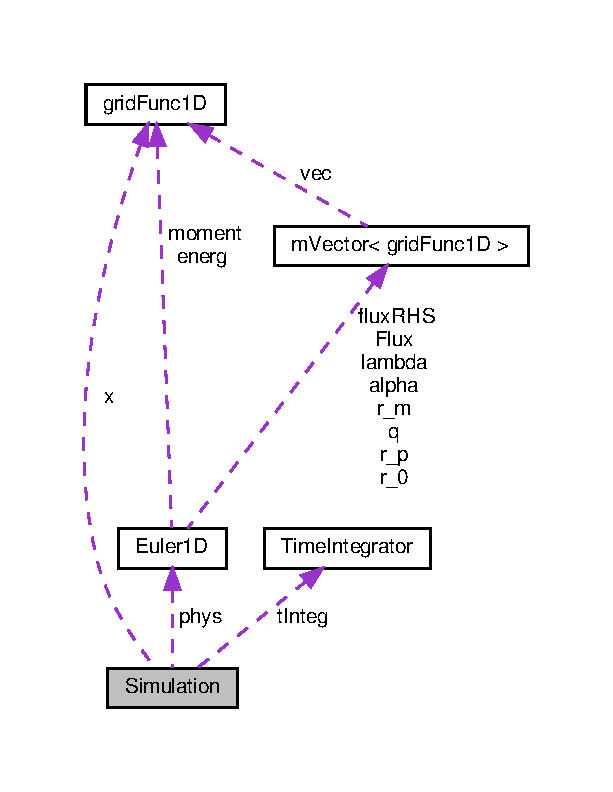
\includegraphics[width=294pt]{classSimulation__coll__graph}
\end{center}
\end{figure}
\subsection*{Public Member Functions}
\begin{DoxyCompactItemize}
\item 
\mbox{\Hypertarget{classSimulation_a895ff3188084f3b63238600cf9cd8659}\label{classSimulation_a895ff3188084f3b63238600cf9cd8659}} 
{\bfseries Simulation} (const \hyperlink{classparameterReader}{parameter\+Reader} \&p)
\item 
\mbox{\Hypertarget{classSimulation_a2ee5c72ad5435c5defa6524e2aae45dd}\label{classSimulation_a2ee5c72ad5435c5defa6524e2aae45dd}} 
void {\bfseries initial\+Data} (const \hyperlink{classparameterReader}{parameter\+Reader} \&p)
\item 
\mbox{\Hypertarget{classSimulation_a0892ba78c1bc7286488761b4fca76c52}\label{classSimulation_a0892ba78c1bc7286488761b4fca76c52}} 
void {\bfseries evolve} ()
\end{DoxyCompactItemize}
\subsection*{Protected Attributes}
\begin{DoxyCompactItemize}
\item 
\mbox{\Hypertarget{classSimulation_a33c150f15bbe3345522eba79bd1e8f33}\label{classSimulation_a33c150f15bbe3345522eba79bd1e8f33}} 
const double \hyperlink{classSimulation_a33c150f15bbe3345522eba79bd1e8f33}{fudge}
\begin{DoxyCompactList}\small\item\em A small quantity. \end{DoxyCompactList}\item 
\mbox{\Hypertarget{classSimulation_a92fd8cd6f62935dd3915e6a1dd6eb4ac}\label{classSimulation_a92fd8cd6f62935dd3915e6a1dd6eb4ac}} 
int \hyperlink{classSimulation_a92fd8cd6f62935dd3915e6a1dd6eb4ac}{n\+\_\+points\+\_\+x}
\begin{DoxyCompactList}\small\item\em Number of points in the x direction. \end{DoxyCompactList}\item 
\mbox{\Hypertarget{classSimulation_a67fda8e9da3b2bbc39545dfc4afa9873}\label{classSimulation_a67fda8e9da3b2bbc39545dfc4afa9873}} 
double \hyperlink{classSimulation_a67fda8e9da3b2bbc39545dfc4afa9873}{x\+Min}
\begin{DoxyCompactList}\small\item\em Minimum value of x coordinate. \end{DoxyCompactList}\item 
\mbox{\Hypertarget{classSimulation_a3c748d2b081bc1c979cc974f420e90ea}\label{classSimulation_a3c748d2b081bc1c979cc974f420e90ea}} 
double \hyperlink{classSimulation_a3c748d2b081bc1c979cc974f420e90ea}{x\+Max}
\begin{DoxyCompactList}\small\item\em Maximum value of x coordinate. \end{DoxyCompactList}\item 
\mbox{\Hypertarget{classSimulation_a6af2df81dac27c93eb75b29c92855049}\label{classSimulation_a6af2df81dac27c93eb75b29c92855049}} 
double \hyperlink{classSimulation_a6af2df81dac27c93eb75b29c92855049}{C\+FL}
\begin{DoxyCompactList}\small\item\em Courant-\/\+Friederich-\/\+Levy factor. \end{DoxyCompactList}\item 
\mbox{\Hypertarget{classSimulation_ae3af859b6e8d5fd02c9f4afaeff54e2a}\label{classSimulation_ae3af859b6e8d5fd02c9f4afaeff54e2a}} 
double \hyperlink{classSimulation_ae3af859b6e8d5fd02c9f4afaeff54e2a}{final\+Time}
\begin{DoxyCompactList}\small\item\em Final time, where simulation stops. \end{DoxyCompactList}\item 
\mbox{\Hypertarget{classSimulation_a898090da97cdad9a7715bf2ec078bfa5}\label{classSimulation_a898090da97cdad9a7715bf2ec078bfa5}} 
double \hyperlink{classSimulation_a898090da97cdad9a7715bf2ec078bfa5}{out\+Every\+Time}
\begin{DoxyCompactList}\small\item\em How often in time we do output. \end{DoxyCompactList}\item 
\mbox{\Hypertarget{classSimulation_a838684076d88a5e923c35c513a1d676c}\label{classSimulation_a838684076d88a5e923c35c513a1d676c}} 
double \hyperlink{classSimulation_a838684076d88a5e923c35c513a1d676c}{time}
\begin{DoxyCompactList}\small\item\em The time coordinate (variable) \end{DoxyCompactList}\item 
\mbox{\Hypertarget{classSimulation_a26f1d3168ba61738b6539537fa95fe3b}\label{classSimulation_a26f1d3168ba61738b6539537fa95fe3b}} 
double \hyperlink{classSimulation_a26f1d3168ba61738b6539537fa95fe3b}{dx}
\begin{DoxyCompactList}\small\item\em Separation between points in x. \end{DoxyCompactList}\item 
\mbox{\Hypertarget{classSimulation_af43e498bfc83c777db5f5ac4025ff923}\label{classSimulation_af43e498bfc83c777db5f5ac4025ff923}} 
double \hyperlink{classSimulation_af43e498bfc83c777db5f5ac4025ff923}{dt}
\begin{DoxyCompactList}\small\item\em Separation between points in time. \end{DoxyCompactList}\item 
\mbox{\Hypertarget{classSimulation_a2b9ba6896919e029f314cafdd0f496ac}\label{classSimulation_a2b9ba6896919e029f314cafdd0f496ac}} 
int \hyperlink{classSimulation_a2b9ba6896919e029f314cafdd0f496ac}{out\+Every}
\begin{DoxyCompactList}\small\item\em How many iterations we do output. \end{DoxyCompactList}\item 
\mbox{\Hypertarget{classSimulation_a592c3b6538cbd268fc31aa806cdddef5}\label{classSimulation_a592c3b6538cbd268fc31aa806cdddef5}} 
int \hyperlink{classSimulation_a592c3b6538cbd268fc31aa806cdddef5}{I\+T\+M\+AX}
\begin{DoxyCompactList}\small\item\em Maximum nunmber of iterations, when simulation stops. \end{DoxyCompactList}\item 
\mbox{\Hypertarget{classSimulation_adb5a7b5d86b920135fb2bf2a0d9516e0}\label{classSimulation_adb5a7b5d86b920135fb2bf2a0d9516e0}} 
\hyperlink{classgridFunc1D}{grid\+Func1D} \hyperlink{classSimulation_adb5a7b5d86b920135fb2bf2a0d9516e0}{x}
\begin{DoxyCompactList}\small\item\em x coordinate \end{DoxyCompactList}\item 
\mbox{\Hypertarget{classSimulation_a801473291b7cf8bf290192383db659e1}\label{classSimulation_a801473291b7cf8bf290192383db659e1}} 
\hyperlink{classEuler1D}{Euler1D} $\ast$ \hyperlink{classSimulation_a801473291b7cf8bf290192383db659e1}{phys}
\begin{DoxyCompactList}\small\item\em The physical system of equations. \end{DoxyCompactList}\item 
\mbox{\Hypertarget{classSimulation_aeee15f5e02978c9b1d3a363e3d6a3800}\label{classSimulation_aeee15f5e02978c9b1d3a363e3d6a3800}} 
\hyperlink{classTimeIntegrator}{Time\+Integrator} \hyperlink{classSimulation_aeee15f5e02978c9b1d3a363e3d6a3800}{t\+Integ}
\begin{DoxyCompactList}\small\item\em The time integration algorithm. \end{DoxyCompactList}\end{DoxyCompactItemize}


\subsection{Detailed Description}


Definition at line 11 of file simulation.\+cpp.



The documentation for this class was generated from the following file\+:\begin{DoxyCompactItemize}
\item 
simulation.\+cpp\end{DoxyCompactItemize}

\hypertarget{classTimeIntegrator}{}\section{Time\+Integrator Class Reference}
\label{classTimeIntegrator}\index{Time\+Integrator@{Time\+Integrator}}
\subsection*{Public Member Functions}
\begin{DoxyCompactItemize}
\item 
\mbox{\Hypertarget{classTimeIntegrator_a149210898e4a69f72e976073d6a17deb}\label{classTimeIntegrator_a149210898e4a69f72e976073d6a17deb}} 
void \hyperlink{classTimeIntegrator_a149210898e4a69f72e976073d6a17deb}{integrate} (\hyperlink{classEuler1D}{Euler1D} \&, double, double)
\begin{DoxyCompactList}\small\item\em Advance the state vector in time one time step. \end{DoxyCompactList}\end{DoxyCompactItemize}


\subsection{Detailed Description}


Definition at line 6 of file time\+Integrator.\+hpp.



The documentation for this class was generated from the following files\+:\begin{DoxyCompactItemize}
\item 
time\+Integrator.\+hpp\item 
time\+Integrator.\+cpp\end{DoxyCompactItemize}

%--- End generated contents ---

% Index
\backmatter
\newpage
\phantomsection
\clearemptydoublepage
\addcontentsline{toc}{chapter}{Index}
\printindex

\end{document}
